\begin{center}
\Huge
Potensfunktioner som væksttype
\end{center}

\section*{Potensvækst}
\stepcounter{section}
Vi har set, hvordan lineær vækst udvikler sig, og vi har set, hvordan eksponentiel vækst udvikler sig. Begge dele fremgår af Fig. \ref{fig:lineks}.
\begin{figure}[H]
\centering
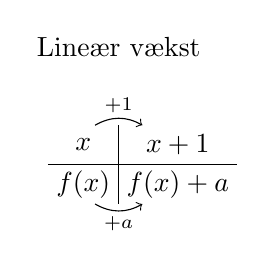
\begin{tikzpicture}
\node at (0,2) {Lineær vækst};
\foreach \i in {0}{
\draw (\i*0.9,0) -- (\i*0.9,1);
}
\draw (-0.9,0.5) -- (1.5,0.5);
\foreach \i in {0}{
\node at (\i*0.9+ 0.75,0.75) {$x+1$};
\node at (\i*0.9+0.75,0.25) {$f(x)+a$};
}
\node at (-0.45,0.75) {$x$};
\node at (-0.45,0.25) {$f(x)$};
\foreach \i in {0}{
\draw [->] (\i*0.9-0.3,1) to [out=30,in=150] (\i*0.9+0.3,1);
\node at (\i*0.9,1.25) {$\scriptstyle+1$};
\draw [->] (\i*0.9-0.3,-0) to [out=-30,in=-150] (\i*0.9+0.3,-0);
\node at (\i*0.9,-0.25) {$\scriptstyle+a$};
}
\end{tikzpicture}
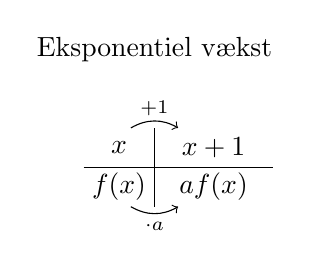
\begin{tikzpicture}
\node at (0,2) {Eksponentiel vækst};
\foreach \i in {0}{
\draw (\i*0.9,0) -- (\i*0.9,1);
}
\draw (-0.9,0.5) -- (1.5,0.5);
\foreach \i in {0}{
\node at (\i*0.9+ 0.75,0.75) {$x+1$};
\node at (\i*0.9+0.75,0.25) {$af(x)$};
}
\node at (-0.45,0.75) {$x$};
\node at (-0.45,0.25) {$f(x)$};
\foreach \i in {0}{
\draw [->] (\i*0.9-0.3,1) to [out=30,in=150] (\i*0.9+0.3,1);
\node at (\i*0.9,1.25) {$\scriptstyle+1$};
\draw [->] (\i*0.9-0.3,-0) to [out=-30,in=-150] (\i*0.9+0.3,-0);
\node at (\i*0.9,-0.25) {$\scriptstyle\cdot a$};
}
\end{tikzpicture}
\caption{Udvikling af lineær og eksponentiel vækst}
\label{fig:lineks}
\end{figure}
Vi kan desværre ikke få noget helt tilsvarende for potensvækst, da en øgning af $x$ med en vil give forskellige fremskrivninger af $f(x)$ alt efter hvad $x$ er. Vi kan derimod beskrive potensvækst ved følgende sætning.
\begin{setn}
Lad $f$ være en potensfunktion, altså 
\begin{align*}
f(x) = b\cdot a^x.
\end{align*}
Så vil en multiplikation af $x$ med en faktor $k$ tilsvare en stigning af $f(x)$ med en faktor $k^a$. Mere præcist gælder der, at 
\begin{align*}
f(k\cdot x) = k^a\cdot f(x).
\end{align*}
\end{setn}
\begin{proof}
Vi betragter 
\begin{align*}
f(k\cdot x) = b\cdot (k\cdot x)^a = b \cdot k^a \cdot x^a = k^a\cdot\underbrace{b\cdot x^a}_{=f(x)} = k^a \cdot f(x),
\end{align*}
hvilket beviser sætningen. 
\end{proof}
Det er værd at bemærke, at det at gange med $k$ tilsvarer at øge $x$ med $(k-1)\cdot 100 \%.$ Tilsvarende svarer multiplikation med $k^a$ til at øge $f(x)$ med $(k^a-1)\cdot 100\%$, så når vi øger $x$ med en hvis procent, så fås en tilsvarende procentvis øgning til $f(x)$. Derfor kaldes potensvækst til tider for $\%\%$-vækst. Lineær vækst kaldes til tider for $\Delta\Delta$-vækst og eksponentiel vækst kaldes til tider for $\Delta\%$-vækst. Potensvækst illustreres på Figur \ref{fig:potens}.
\begin{figure}[H]
\centering
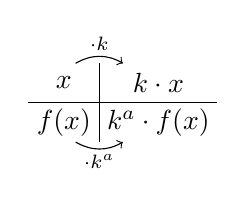
\begin{tikzpicture}
\foreach \i in {0}{
\draw (\i*0.9,0) -- (\i*0.9,1);
}
\draw (-0.9,0.5) -- (1.5,0.5);
\foreach \i in {0}{
\node at (\i*0.9+ 0.75,0.75) {$k\cdot x$};
\node at (\i*0.9+0.75,0.25) {$k^a \cdot f(x)$};
}
\node at (-0.45,0.75) {$x$};
\node at (-0.45,0.25) {$f(x)$};
\foreach \i in {0}{
\draw [->] (\i*0.9-0.3,1) to [out=30,in=150] (\i*0.9+0.3,1);
\node at (\i*0.9,1.25) {$\scriptstyle\cdot k$};
\draw [->] (\i*0.9-0.3,-0) to [out=-30,in=-150] (\i*0.9+0.3,-0);
\node at (\i*0.9,-0.25) {$\scriptstyle\cdot k^a$};
}
\end{tikzpicture}
\caption{Udvikling af potensvækst}
\label{fig:potens}
\end{figure}

\begin{exa}
	Arealet af et rektangel med højde $2x$ og bredde $x$ har vi tidligere set kunne beskrives 
	ved potensfunktionen $A$ givet ved
	\begin{align*}
		A(x) = 2x^2.
	\end{align*}
	Hvis $x = 2$, så er bredden $2$, højden 4 og arealet 8. Tilsvarende giver $x = 4$ os 
	bredden 4, højden 8 og arealet 32. Dette kan ses på Figur \ref{fig:rektangler}.
	\begin{figure}[H]
		\centering
		\begin{tikzpicture}
			%Småt rektangel
			\draw[fill = teal] (-2,-2) rectangle (0,2);
			\draw[decorate,	decoration = {calligraphic brace, mirror, raise = 3pt, amplitude = 5pt}, thick, pen colour = {teal}] (-2,-2) --  (0,-2);
			\draw[decorate,	decoration = {calligraphic brace, raise = 3pt, amplitude = 5pt}, thick, pen colour = {teal}] (-2,-2) --  (-2,2);
			\node[color = teal] at (-1,-2.6) {2};
			\node[color = teal] at (-2.5,0) {4};
			%Stort rektangel:
			\draw[fill = purple] (1,-2) rectangle (5,6);
			\draw[dashed, thick] (3,-2) -- (3,2);
			\draw[dashed, thick] (3,2) -- (1,2);
			\draw[decorate,	decoration = {calligraphic brace, mirror, raise = 3pt, amplitude = 5pt}, thick, pen colour = {purple}] (1,-2) --  (5,-2);
			\draw[decorate,	decoration = {calligraphic brace, mirror, raise = 3pt, amplitude = 5pt}, thick, pen colour = {purple}] (5,-2) --  (5,6);
			\node[color = purple] at (3,-2.6) {4};
			\node[color = purple] at (5.5,2) {8};
			%Legend:
			\draw[fill = purple, draw = none] (6,-2) rectangle (6.3,-1.7);
			\draw[fill = teal, draw = none] (6,-1) rectangle (6.3,-0.7); 		 			
			\node[color = purple, anchor = west] at (6.4, -1.85) { = 32};
			\node[color = teal, anchor = west] at (6.4, -0.85) { = 8};
		\end{tikzpicture}
		\caption{To ligedannede rektangler}
		\label{fig:rektangler}
	\end{figure}
	Dette passer også med vores forventning, da ved at gange vores $x$-værdi med 2 (2 til 4)
	gør, at vi skal gange vores samlede areal med $2^a = 2^2 = 4$, hvilket som kan ses af 
	Figur \ref{fig:rektangler} er fra 8 til 32.
\end{exa}

\subsection*{Opgave 1}
\begin{enumerate}[label = \roman*)]
	\item Gang sidelængden i rektanglet med 3, så $x = 6$. Hvor mange gange større bliver arealet?
	\item Gang sidelængden i rektanglet med 4, så $x = 8$. Hvor mange gange større bliver arealet?
	\item Gang sidelængden i rektanglet med 5, så $x = 10$. Hvor mange gange større bliver arealet?
\end{enumerate}

\subsection*{Opgave 2}
En kasse har længde, højde og bredde $x$. 
\begin{enumerate}[label=\roman*)]
	\item Bestem forskriften for den potensfunktion $f$, der beskriver rumfanget af kassen.
	\item Bestem rumfanget, hvis $x = 2$.
	\item Gang sidelængden med $2$, så $x = 4$. Hvor mange gange større bliver rumfanget?
	\item Gang sidelængden med $3$, så $x = 6$. Hvor mange gange større bliver rumfanget?
	\item Gang sidelængden med $4$, så $x = 8$. Hvor mange gange større bliver rumfanget?
	\item Gang sidelængden med $5$, så $x = 10$. Hvor mange gange større bliver rumfanget?
\end{enumerate}

\subsection*{Opgave 3}
En trekant har højde og grundlinje $x$. 
\begin{enumerate}[label = \roman*)]
	\item Bestem forskriften for den potensfunktion, der beskriver arealet af trekanten
	\item Bestem arealet, hvis $x = 2$.
	\item Gang sidelængden med $2$, så $x = 4$. Hvor mange gange større bliver arealet?
	\item Gang sidelængden med $3$, så $x = 6$. Hvor mange gange større bliver arealet?
	\item Gang sidelængden med $4$, så $x = 8$. Hvor mange gange større bliver arealet?
	\item Gang sidelængden med $5$, så $x = 10$. Hvor mange gange større bliver arealet?
\end{enumerate}

\subsection*{Opgave 4}
Rumfanget af en kugle med radius $x$ er givet ved
\begin{align*}
	R(x) = \frac{4}{3}\pi x^3.
\end{align*}
\begin{enumerate}[label = \roman*)]
	\item Bestem rumfanget, hvis $x = 2$.
	\item Gang radius med $2$, så $x = 4$. Hvor mange gange større bliver rumfanget?
	\item Gang radius med $3$, så $x = 6$. Hvor mange gange større bliver rumfanget?
	\item Gang radius med $4$, så $x = 8$. Hvor mange gange større bliver rumfanget?
	\item Gang radius med $5$, så $x = 10$. Hvor mange gange større bliver rumfanget?
\end{enumerate}

\subsection*{Opgave 5}
En potensfunktion $f$ er givet ved
\begin{align*}
	f(x) = 5\cdot x^5.
\end{align*}
\begin{enumerate}[label=\roman*)]
	\item Hvad øges funktionsværdien med, hvis $x$ ganges med $2$?
	\item Hvad øges funktionsværdien med, hvis $x$ ganges med $1.5$?
\end{enumerate}

\subsection*{Opgave 6}
En potensfunktion $f$ er givet ved
\begin{align*}
	f(x) = 3 \cdot x^{1.7}
\end{align*}

Udfyld følgende tabel uden at sætte $x$-værdierne ind i forskriften for $f$.
\begin{center}
	\begin{tabular}{c|c|c|c|c|c|c|c}
		$x$ & 1 & 2 & 4 & 5 & 6 & 8 & 11 \\ \hline
		$f(x)$ & 3 & & & & & &
	\end{tabular}
\end{center}

\subsection*{Opgave 7}
Den effekt, det kræves at bevæge sig gennem luft med kan beskrives ved 
\begin{align*}
P(v) = K\cdot v^3,
\end{align*}
hvor $v$ beskriver hastigheden og $K$ er en konstant, der afhænger af en række forhold.
\begin{enumerate}[label=\roman*)]
\item Hvis vi øger hastigheden $v$ med $50\%$, hvor meget øges den effekt, der kræves for at bevæge sig gennem luften så med? 
\item Hvis vi øger vores effekt med $200\%$, hvor meget hurtigere kan vi så bevæge os gennem luften?
\end{enumerate}
\subsection*{Opgave 8}
Bremselængden for en bil kan beskrives ved $D$ givet ved
\begin{align*}
D(v) = k\cdot v^2.
\end{align*}
\begin{enumerate}[label=\roman*)]
\item Hvis vi øger hastigheden med $20\%$, hvor meget øges bremselængden $D$ så med?
\item Hvis vi vil sænke vores bremselængde med $50\%$, hvor meget skal vi så sænke vores hastighed med?
\end{enumerate}


